% Created 2022-04-29 Fr 21:49
% Intended LaTeX compiler: pdflatex
\documentclass[letterpaper, 11pt]{article}
\usepackage[utf8]{inputenc}
\usepackage[T1]{fontenc}
\usepackage{graphicx}
\usepackage{grffile}
\usepackage{longtable}
\usepackage{wrapfig}
\usepackage{rotating}
\usepackage[normalem]{ulem}
\usepackage{amsmath}
\usepackage{textcomp}
\usepackage{amssymb}
\usepackage{capt-of}
\usepackage{hyperref}
\usepackage{lmodern} % Ensures we have the right font
\usepackage[T1]{fontenc}
\usepackage[utf8]{inputenc}
\usepackage{graphicx, breqn}
\usepackage{mathtools, amsthm, amssymb, breqn}
\usepackage[table, xcdraw]{xcolor}
\definecolor{bblue}{HTML}{0645AD}
\usepackage[colorlinks]{hyperref}
\hypersetup{colorlinks, linkcolor=blue, urlcolor=bblue}
\usepackage{titling}
\setlength{\droptitle}{-6em}
\setlength{\parindent}{0pt}
\setlength{\parskip}{1em}
\usepackage[stretch=10]{microtype}
\usepackage{hyphenat}
\usepackage{ragged2e}
\usepackage{subfig} % Subfigures (not needed in Org I think)
\usepackage{hyperref} % Links
\usepackage{listings} % Code highlighting
\usepackage{pgfplots} % Plotting graphs
\usepackage{efbox}
\usepackage{tikz}
\usepackage{onimage} % note that onimage.sty must be in the working directory.
\usepackage[top=1in, bottom=1.25in, left=1.55in, right=1.55in]{geometry}
\renewcommand{\baselinestretch}{1.15}
\usepackage[explicit]{titlesec}
\pretitle{\begin{center}\fontsize{20pt}{20pt}\selectfont}
\posttitle{\par\end{center}}
\preauthor{\begin{center}\vspace{-6bp}\fontsize{14pt}{14pt}\selectfont}
\postauthor{\par\end{center}\vspace{-25bp}}
\predate{\begin{center}\fontsize{12pt}{12pt}\selectfont}
\postdate{\par\end{center}\vspace{0em}}
\titlespacing\section{0pt}{5pt}{5pt} % left margin, space before section header, space after section header
\titlespacing\subsection{0pt}{5pt}{-2pt} % left margin, space before subsection header, space after subsection header
\titlespacing\subsubsection{0pt}{5pt}{-2pt} % left margin, space before subsection header, space after subsection header
\usepackage{enumitem}
\setlist{itemsep=-2pt} % or \setlist{noitemsep} to leave space around whole list
\usepackage {mathtools , amssymb , amsthm}
\author{Fred Mitchell}
\date{\today}
\title{Slit Scan -- Generate an effect similar to 2001's star gate sequences}
\hypersetup{
 pdfauthor={Fred Mitchell},
 pdftitle={Slit Scan -- Generate an effect similar to 2001's star gate sequences},
 pdfkeywords={},
 pdfsubject={},
 pdfcreator={Emacs 28.1 (Org mode 9.1.5)}, 
 pdflang={English}}
\begin{document}

\maketitle
\tableofcontents


\section{Fundamentals and Design}
\label{sec:orge63da78}
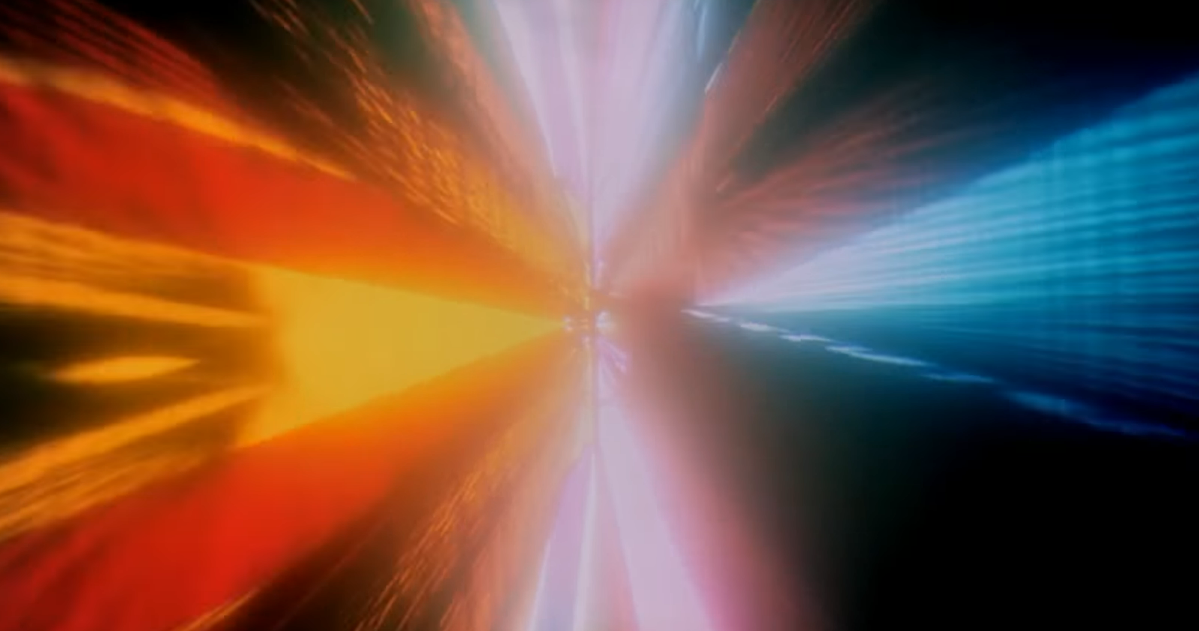
\includegraphics[scale=0.4]{images/2001-example.png}
\subsection{Introduction}
\label{sec:org88b0d0c}
Slit-Scan is the command-line tool that allow you to create slit-scans similar to
the star-gate sequences in 2001: A Space Odyssey. The idea here is to add a lot of flexibility
to allow you to acheive results even beyond what was acheived in what is arguably the greatest
Science Fiction film of all time.
\subsection{Mathematics}
\label{sec:org50badca}
Here, we fully specify the mathematics involved with the slit-scan function.

\subsubsection{Generating the slit}
\label{sec:orgfade46a}
Firstly, we define the slit function as a function between 2 points.

\item $t$ is time, in seconds, and
\item $p_1, p_2$ are points defining tbe beginning and ending of the slit, and
\item $$
 slit(p_1, p_2, \rho) = g(p_1, p_2, curve(\rho)) \Bigr| _{\rho=0} ^{\rho=1}
$$
\item where $$
 \begin{array}{l}
 p_1 = (x_1, y_1)\\
 p_2 = (x_2, y_2)
 \end{array}
$$
\item and $0 \ge x, y, \rho \ge 1$

where \(curve(\rho)\) defines the shape of the slit. For the traditional case,
\(curve(\rho)\) will be \(0\), defining a straight line from \(p_1\) to \(p_2\). In other cases,
\(curve(\rho)\) will result in pertubations in the \((p_1, p_2)\) line, perpendular to the
line itself.

\(\rho\) is the parametic for the slit. \(x\) and \(y\) represnts the idealized coordinates of the
image being scanned by the slit, which will be converted to the actual physical coordinates of
the pixels in the image, along with pixel averaging in the 3x3 or 5x5 square with the physical
coordinate being at the center.

Secondly, we define the movement of the slit across an image in terms of time \(t\) (in seconds):

$$
\begin{array}{l}
    p_1{_t} = p_1(t)\\
    p_2{_t} = p_2(t)
\end{array}
$$

Where said movement of \(p_1\) and \(p_2\) may be independent with each other, solely with \(t\) as their
common parametric basis, but in most cases the "trivial" or traditional approach will be taken as the 
movenent being equivalent, basically to "scan" the image from one side to the other.

Thirdly, we define the compositor function. The compositor is responsible for compositing the time-varying
contents of the slit unto the final canvas. Here, the canvas is bisected either horizontally or vertically
by a straight-line slit, and with each time instant, the slit contents is forwarded away from the slit.

\begin{itemize}
\item The Hip library provides a way to navagate the image via
map functions. The imap provides (x,y) coordinates
of the pixels given. We can and will problably have
to do do some sort of lookup "table" on the coordinates
to perform the expected operation, but I need to 
give this more thought.
\end{itemize}

\subsubsection{The Compositor}
\label{sec:orga8b8d2f}
The compositor may "stretch" the contents of the slit as a function of the distance from the slit until it
reaches the end of the canvass.

\tikzset{annotations/.style = {
  tsx/show help lines,
  every path/.append style = {very thick, color = red},
  every node/.append style = {blue, font = \bfseries\sffamily}}}

\begin{tikzonimage}[width=.8\textwidth]{images/compositor.png}
  [annotations]
  \draw (0.3,0.5) edge[->] (0.1,0.9) (0.73,0.4) edge[->] (0.9,0.9);
  \node[rotate=90] at (0.27,0.3) {canvas};
  \node[rotate=30] at (0.86,0.65) {slit expansion};
\end{tikzonimage}

\begin{tikzpicture}
  \begin{axis} [grid, axis lines=center]
  \addplot [domain=-3:3, thick, smooth] { x^3 - 6*x };
  \end{axis}
\end{tikzpicture}

$$
 \frac{f(x)-f(a) x-a}g
$$

\section{General Documentation and Use of Slit Scan}
\label{sec:org48f2061}
This covers the usage from the command-line. Rather than go into extensive documentation
on the command-line commands and options (the program itself provides this), we shall
give some helpul examples.
\subsection{Simple case -- one image, simple vertical slit}
\label{sec:orgfb5f209}
slit-scan --i1 flower.jpg --format png --out film/

\subsection{Typical -- 2 images simple vertical and horizontal slits}
\label{sec:orgbc1f3bf}
\subsection{Advanced 1 -- 2 images, staight line rotating slit}
\label{sec:org6eec87b}
\subsection{Advanced 2 -- 2 images, sine slit}
\label{sec:org1d78aa1}
\subsection{Advanced 3 -- 2 images, rotating sine slit}
\label{sec:org11ac4c1}
\subsection{Advanced 4 -- 2 images, arbitrary function for the slit and the 2 endpoints}
\label{sec:orgac753e6}
\end{document}